\documentclass[10pt, a4paper]{article}

% On écrit en français
\usepackage[utf8]{inputenc}
\usepackage[frenchb]{babel}
\usepackage[T1]{fontenc}

% Packages nécessaires
\usepackage{graphicx}
\usepackage{hyperref}

% Numérotation de page custom
\usepackage{fancyhdr}
\usepackage{lastpage}
\pagestyle{fancy}
\fancyhf{}
\rfoot{Page \thepage \hspace{1pt} sur \pageref{LastPage}}

% Police Helvetica <3
\usepackage{helvet}
\renewcommand*{\familydefault}{\sfdefault}

% Enlever les alinéas
\setlength{\parindent}{0pt}

% Marges plus larges pour faire moins LaTeX
\usepackage[left=3cm, right=3cm]{geometry}

% Sous titre de document
\usepackage{titling}
\newcommand{\subtitle}[1]{%
  \posttitle{%
    \par\end{center}
    \begin{center}\large#1\end{center}
    \vskip0.5em}%
}

% En tête complet de document
\newcommand{\Document}[1]{%
    \title{#1}
    \subtitle{Dématérialisation d'un processus de paiement}
    \author{
        COMETS Jean-Marie \\
        DELMARRE Adrian \\
        REYNOLDS Nicolas \\
        TURPIN Pierre
    }
    \date{\today}

    \maketitle \newpage

    \tableofcontents \newpage
}

\usepackage{wrapfig}
\usepackage{lscape}
\begin{document}

\Document{Expression des besoins}

\section{Objet du projet}

Forte d'une vision particulière et d'une expertise avancée en matière de
transactions sécurisées et ergonomiques, l'entreprise AVENTIX se propose de
concurrencer SODEXHO dans un des domaines qui en ont fait la renommée, en
remplaçant les traditionnels chèques restaurant par des puces NFC. Hormis
l'aspect simple, moderne et ludique du produit, qui semble séduire le
consommateur final d'après les premières études du marché, c'est surtout sur la
simplification drastique du workflow de paiement, de par sa dématérialisation,
qu'AVENTIX compte pour convaincre les différents acteurs du secteur. \\

L'objectif de ce projet est de spécifier le système proposé par AVENTIX dans le
cadre d'une étude préliminaire.

\section{Contexte du projet}

Au jour d'aujourd'hui, la chaîne de traitement des chèques restaurant fait
intervenir cinq acteurs: une société qui émet les chèques restaurant,
l'employeur qui achète les chèques pour les céder aux employés en prenant à sa
charge une partie de valeur indiquée, l'employé qui utilise le chèque et enfin
le commerçant affilié auprès d'une centrale de règlement des titres (CRT). Le
traitement des chèques restaurant est semi-automatique car il nécessite
l'envoi des chèques par les commerçants à la centrale de règlement des titres.
A ce niveau, les chèques sont traités de façon informatique afin de permettre
aux commerçants d'être crédités.

\begin{figure}[h!]
    \centering
    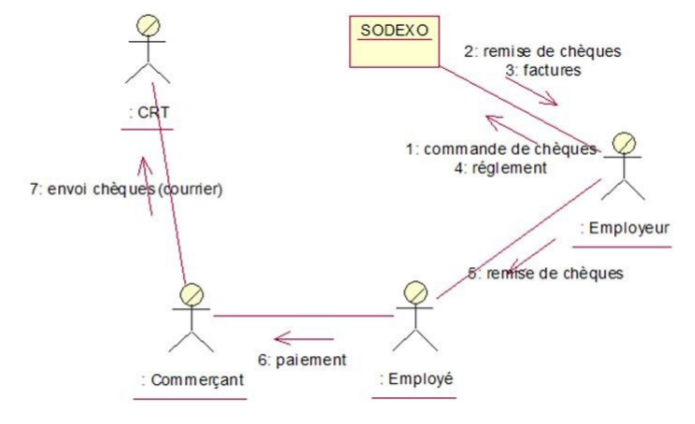
\includegraphics[width=0.8\textwidth]{cdu1}
    \label{fig:cdu1}
\end{figure}

Pour supprimer la partie manuelle dans la chaîne de traitement des chèques
restaurant au profit d'un traitement entièrement automatique, on souhaite
remplacer le chèque par une puce NFC sans que cela modifie, sur le plan de
l'organisation, les procédures d'acquisition et de traitement déjà utilisées.
On nommera ce nouveau mode : carte restaurant. Ainsi, on envisage une
simplification des protocoles d'acquisition et d'utilisation.

\begin{figure}[h!]
    \centering
    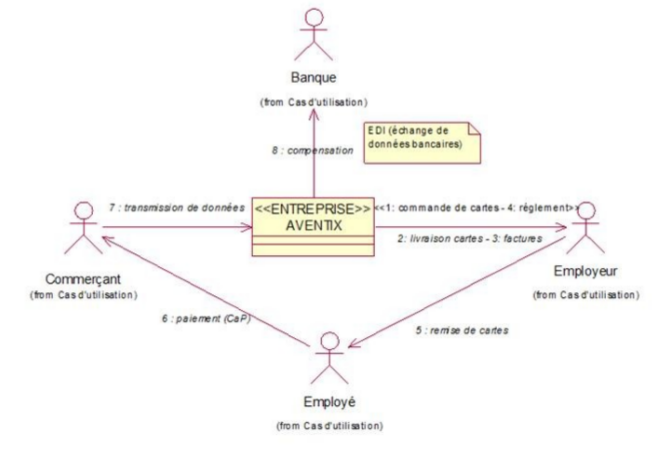
\includegraphics[width=0.8\textwidth]{cdu2}
    \label{fig:cdu2}
\end{figure}

\section{Acteurs}

\subsection{Acteurs externes}

\begin{description}
    \item[Banques] Cet acteur représente les enseignes bancaires garantissant
        la sécurité des transactions (terminaux et internet) et leurs
        échéances.
    \item[Fournisseurs] Cet acteur représente les entreprises fabricant ou
        important les bornes NFC mises en place chez les commerçants
        partenaires.
    \item[Installateurs / maintenance] Cet acteur représente les artisans
        accrédités responsables de la mise en place des bornes NFC chez les
        commerçants partenaires, ainsi que des opérations de maintenance.
    \item[Commerçants] Cet acteur représente les enseignes (restaurants et
        grandes surfaces) qui acceptent la puce NFC comme moyen de paiement
        d'une prestation.
    \item[Entreprise] Cet acteur représente les employeurs qui adhèrent à la
        puce NFC. Il interagit avec le système dans le cadre du processus de
        gestion de commande et du processus de livraison-facturation.
    \item[Borne NFC] Cet acteur modélise un lecteur de puce NFC installé chez
        un commerçant et qui permet de transmettre les données relatives à une
        transaction commerciale.
    \item[Utilisateur final] Cet acteur modélise le client final de la solution
        B2B2C, l'utilisateur de la puce NFC.
\end{description}

\subsection{Acteurs internes}

\begin{description}
    \item[Service commande] Correspond au poste de travail qui traite les
        commandes (saisie, édition et envoi de bons de commande). Cet acteur
        s'occupe également des devis.
    \item[Service facturation] Correspond au poste de travail qui traite les
        factures (élaboration des règles de facturation, édition et ennvoi des
        factures). Cet acteur s'occupe également des expéditions de puces NFC à
        destination des entreprises.
    \item[Service traitement] Correspond au service chargé de surveiller le
        traitement des transactions. Une transaction s'effectue entre un
        commerçant et le système. Ce service est également chargé de mettre à
        jour les données suite aux sollicitations des employeurs ou des
        employés.
    \item[Service marketing] Correspond au service responsable de la
        prospection de nouveaux clients, quelle que soit leur nature, du
        dimensionnement (nombre de bornes, etc.) et de l'établissement de
        contrats.
    \item[Service client] Correspond à l'interface entre les clients
        (entreprises et commerçants), garant de la qualité des services
        proposés et récipendaire des réclamations éventuelles.
\end{description}

\section{Besoins fonctionnels}

\subsection{Attentes de gestion}

\begin{itemize}
    \item Traitement des commandes :
        \begin{itemize}
            \item De crédit (par le truchement de la banque)
            \item D'installation de machines (par le truchement des
                fournisseurs et installateurs)
        \end{itemize}
    \item Édition de factures
\end{itemize}

\subsection{Attentes métier}

\begin{itemize}
    \item Compensation (gestion des transactions) :
        \begin{itemize}
            \item Crédit d'un compte client.
                \begin{itemize}
                    \item Par l'entreprise.
                    \item Par lui-même.
                \end{itemize}
            \item Débit d'un compte client.
                \begin{itemize}
                    \item Par un RIE / RE.
                    \item Par une grande surface.
                    \item Par un enseigne de restauration.
                \end{itemize}
            \item Crédit d'un compte commerçant.
            \item Débit d'un compte commerçant.
        \end{itemize}
\end{itemize}

\subsection{Attentes B2B/B2C}

\begin{itemize}
    \item Marketing :
        \begin{itemize}
            \item Étude de marché : pénétration d'un nouveau mode de
                transaction dans un marché fermé.
                \begin{itemize}
                    \item Auprès des entreprises, qui seraient susceptibles d'y
                        recourir,
                    \item Auprès des utilisateurs finaux, dont l'intérêt
                        justifierait l'investissement pour l'entreprise.
                \end{itemize}
            \item Prospection commerciale : conclusion d'accords de principe //
                démarchage.
                \begin{itemize}
                    \item Auprès des entreprises,
                    \item Auprès des grandes surfaces.
                \end{itemize}
        \end{itemize}
    \item Mise en place d'une interface web destinée aux entreprises voulant
        adhérer au programme ou gérer leur compte.
    \item Mise en place d'une interface web destinée aux utilisateurs finaux
        souhaitant gérer leur crédit.
\end{itemize}

\subsection{Attentes interopérabilité}

\begin{itemize}
    \item Mise en place d'une architecture modulaire et évolutive.
    \item Respect des normes d'usage.
    \item (rétro)compatibilité avec les systèmes existants.
\end{itemize}

\section{Cas d'utilisation}

\begin{landscape}
  \begin{figure}[ht]
      \centering
      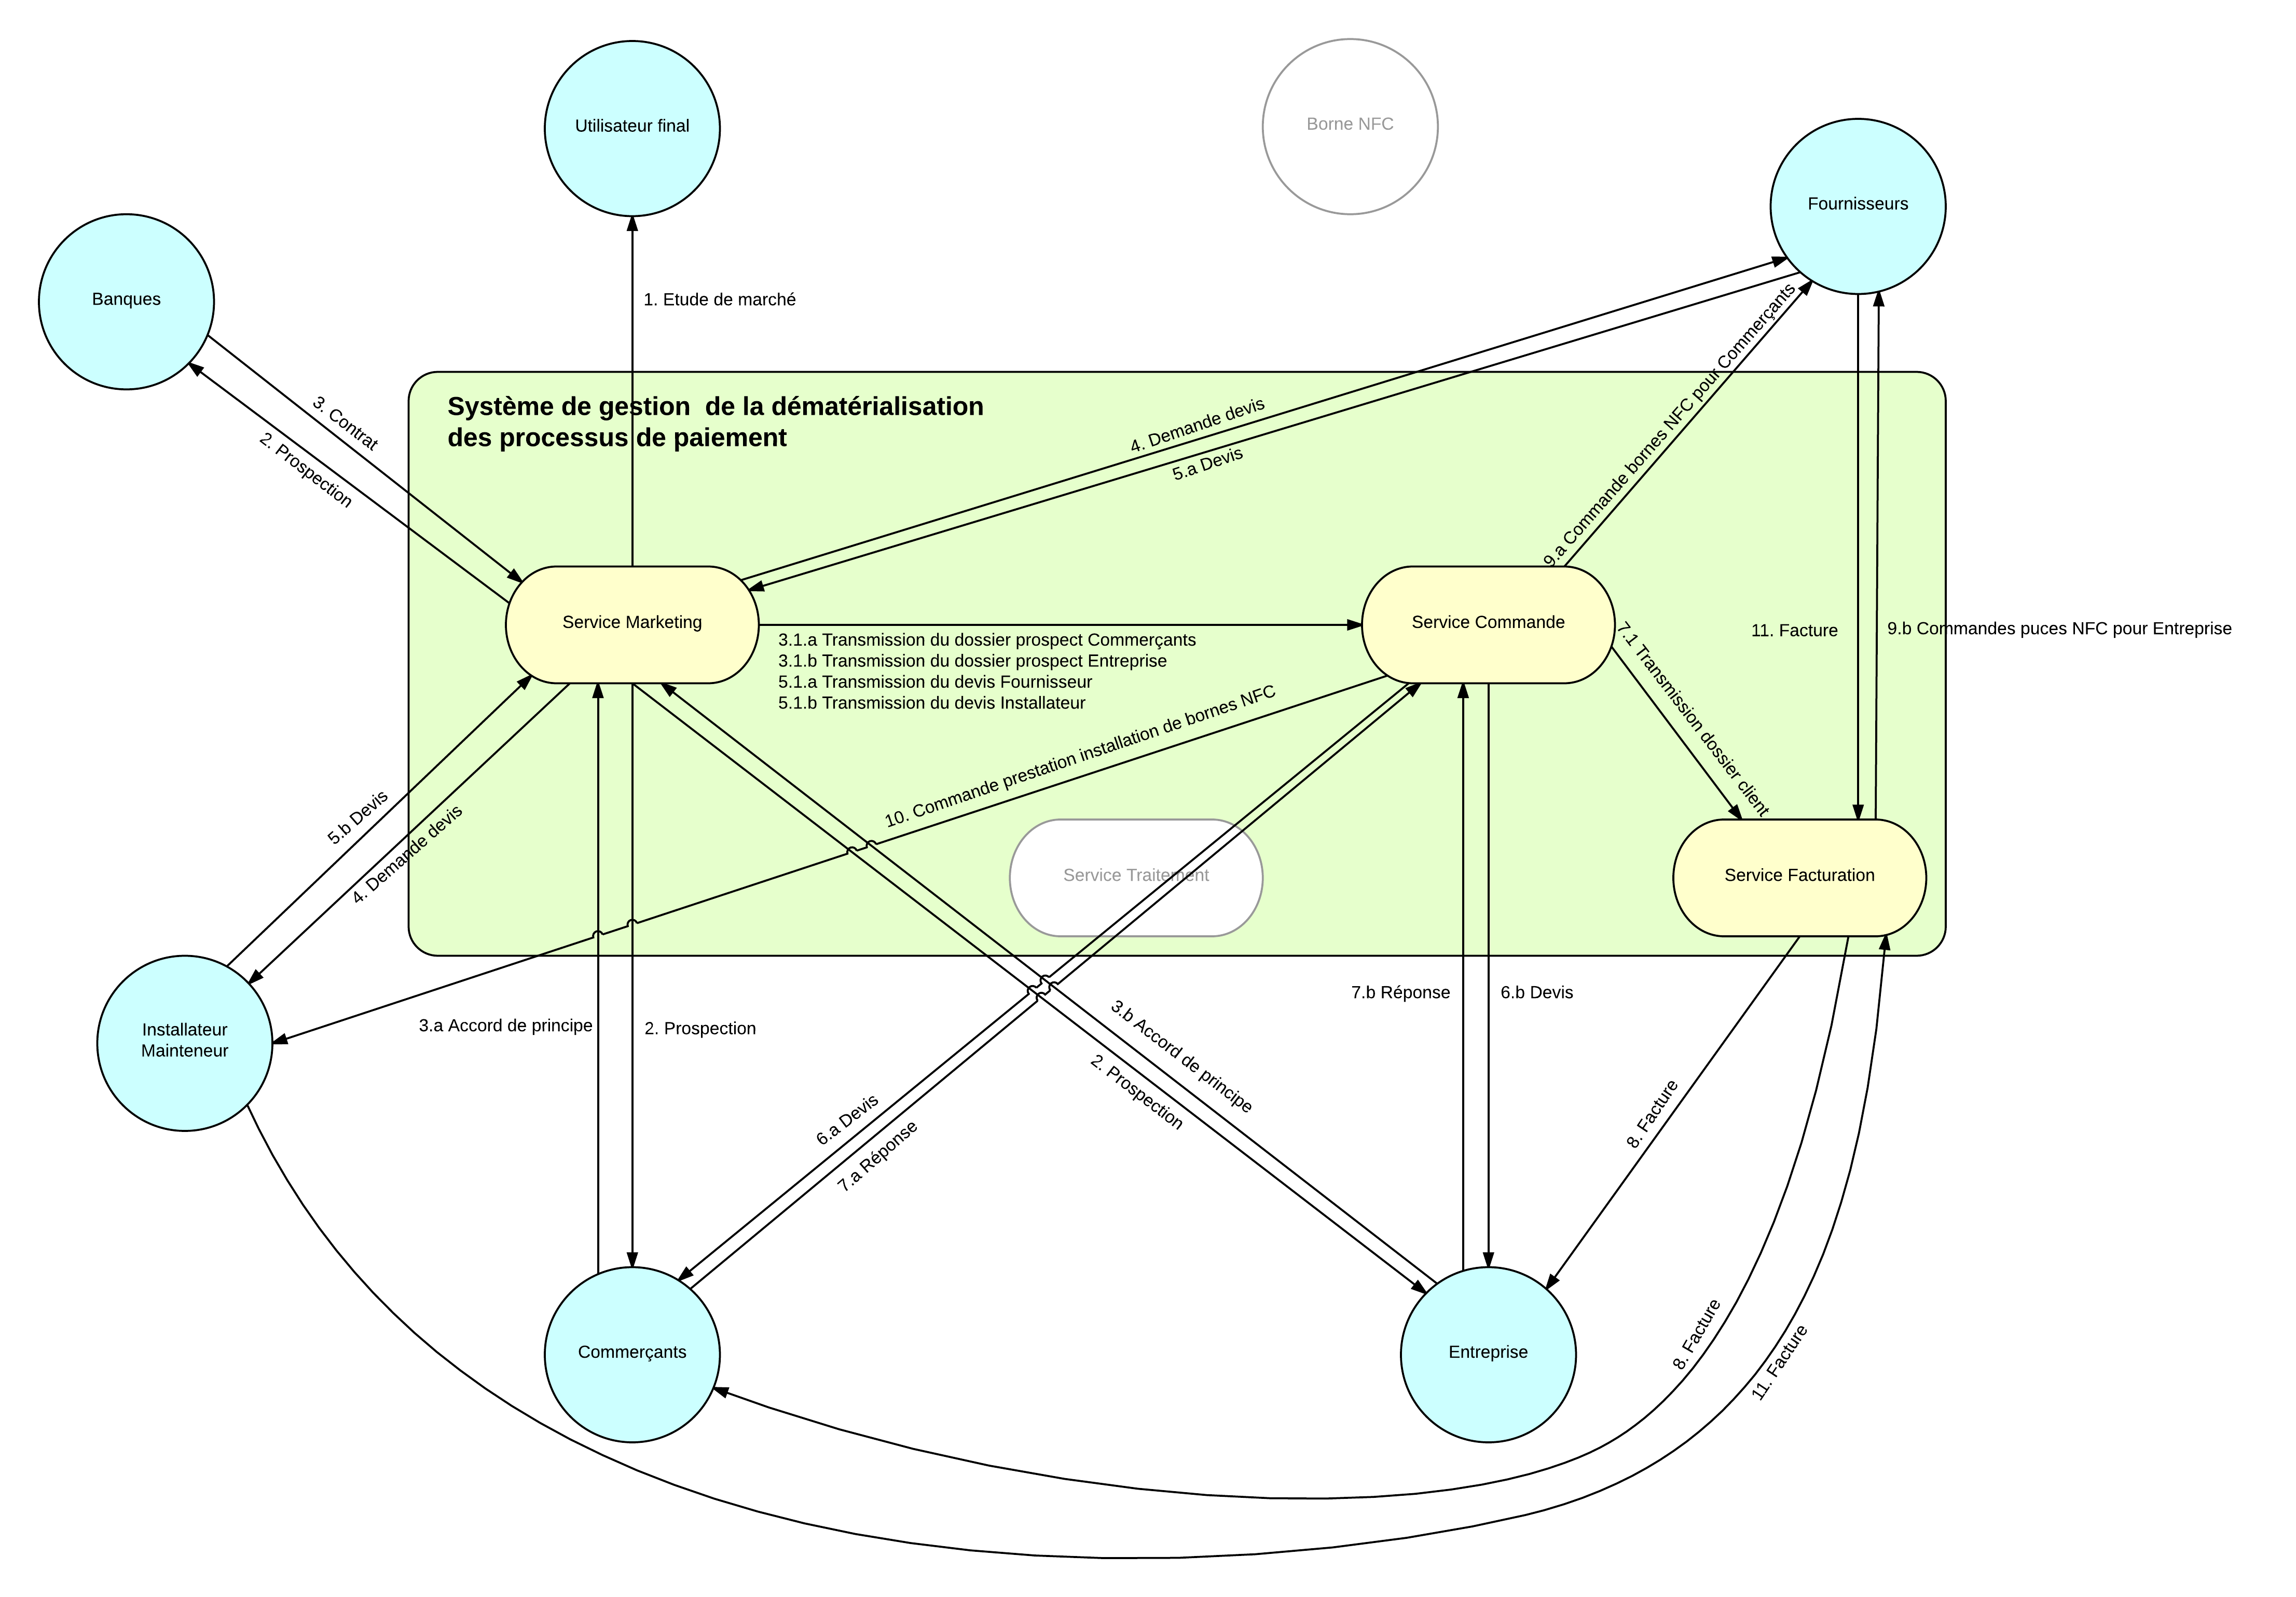
\includegraphics[width=0.7\paperheight]{mcc-marketing}
      \caption{MCC Spécifique au marketing}
      \label{fig:mcc-marketing}
  \end{figure}
\end{landscape}
\newpage

\begin{landscape}
  \begin{figure}[ht]
      \centering
      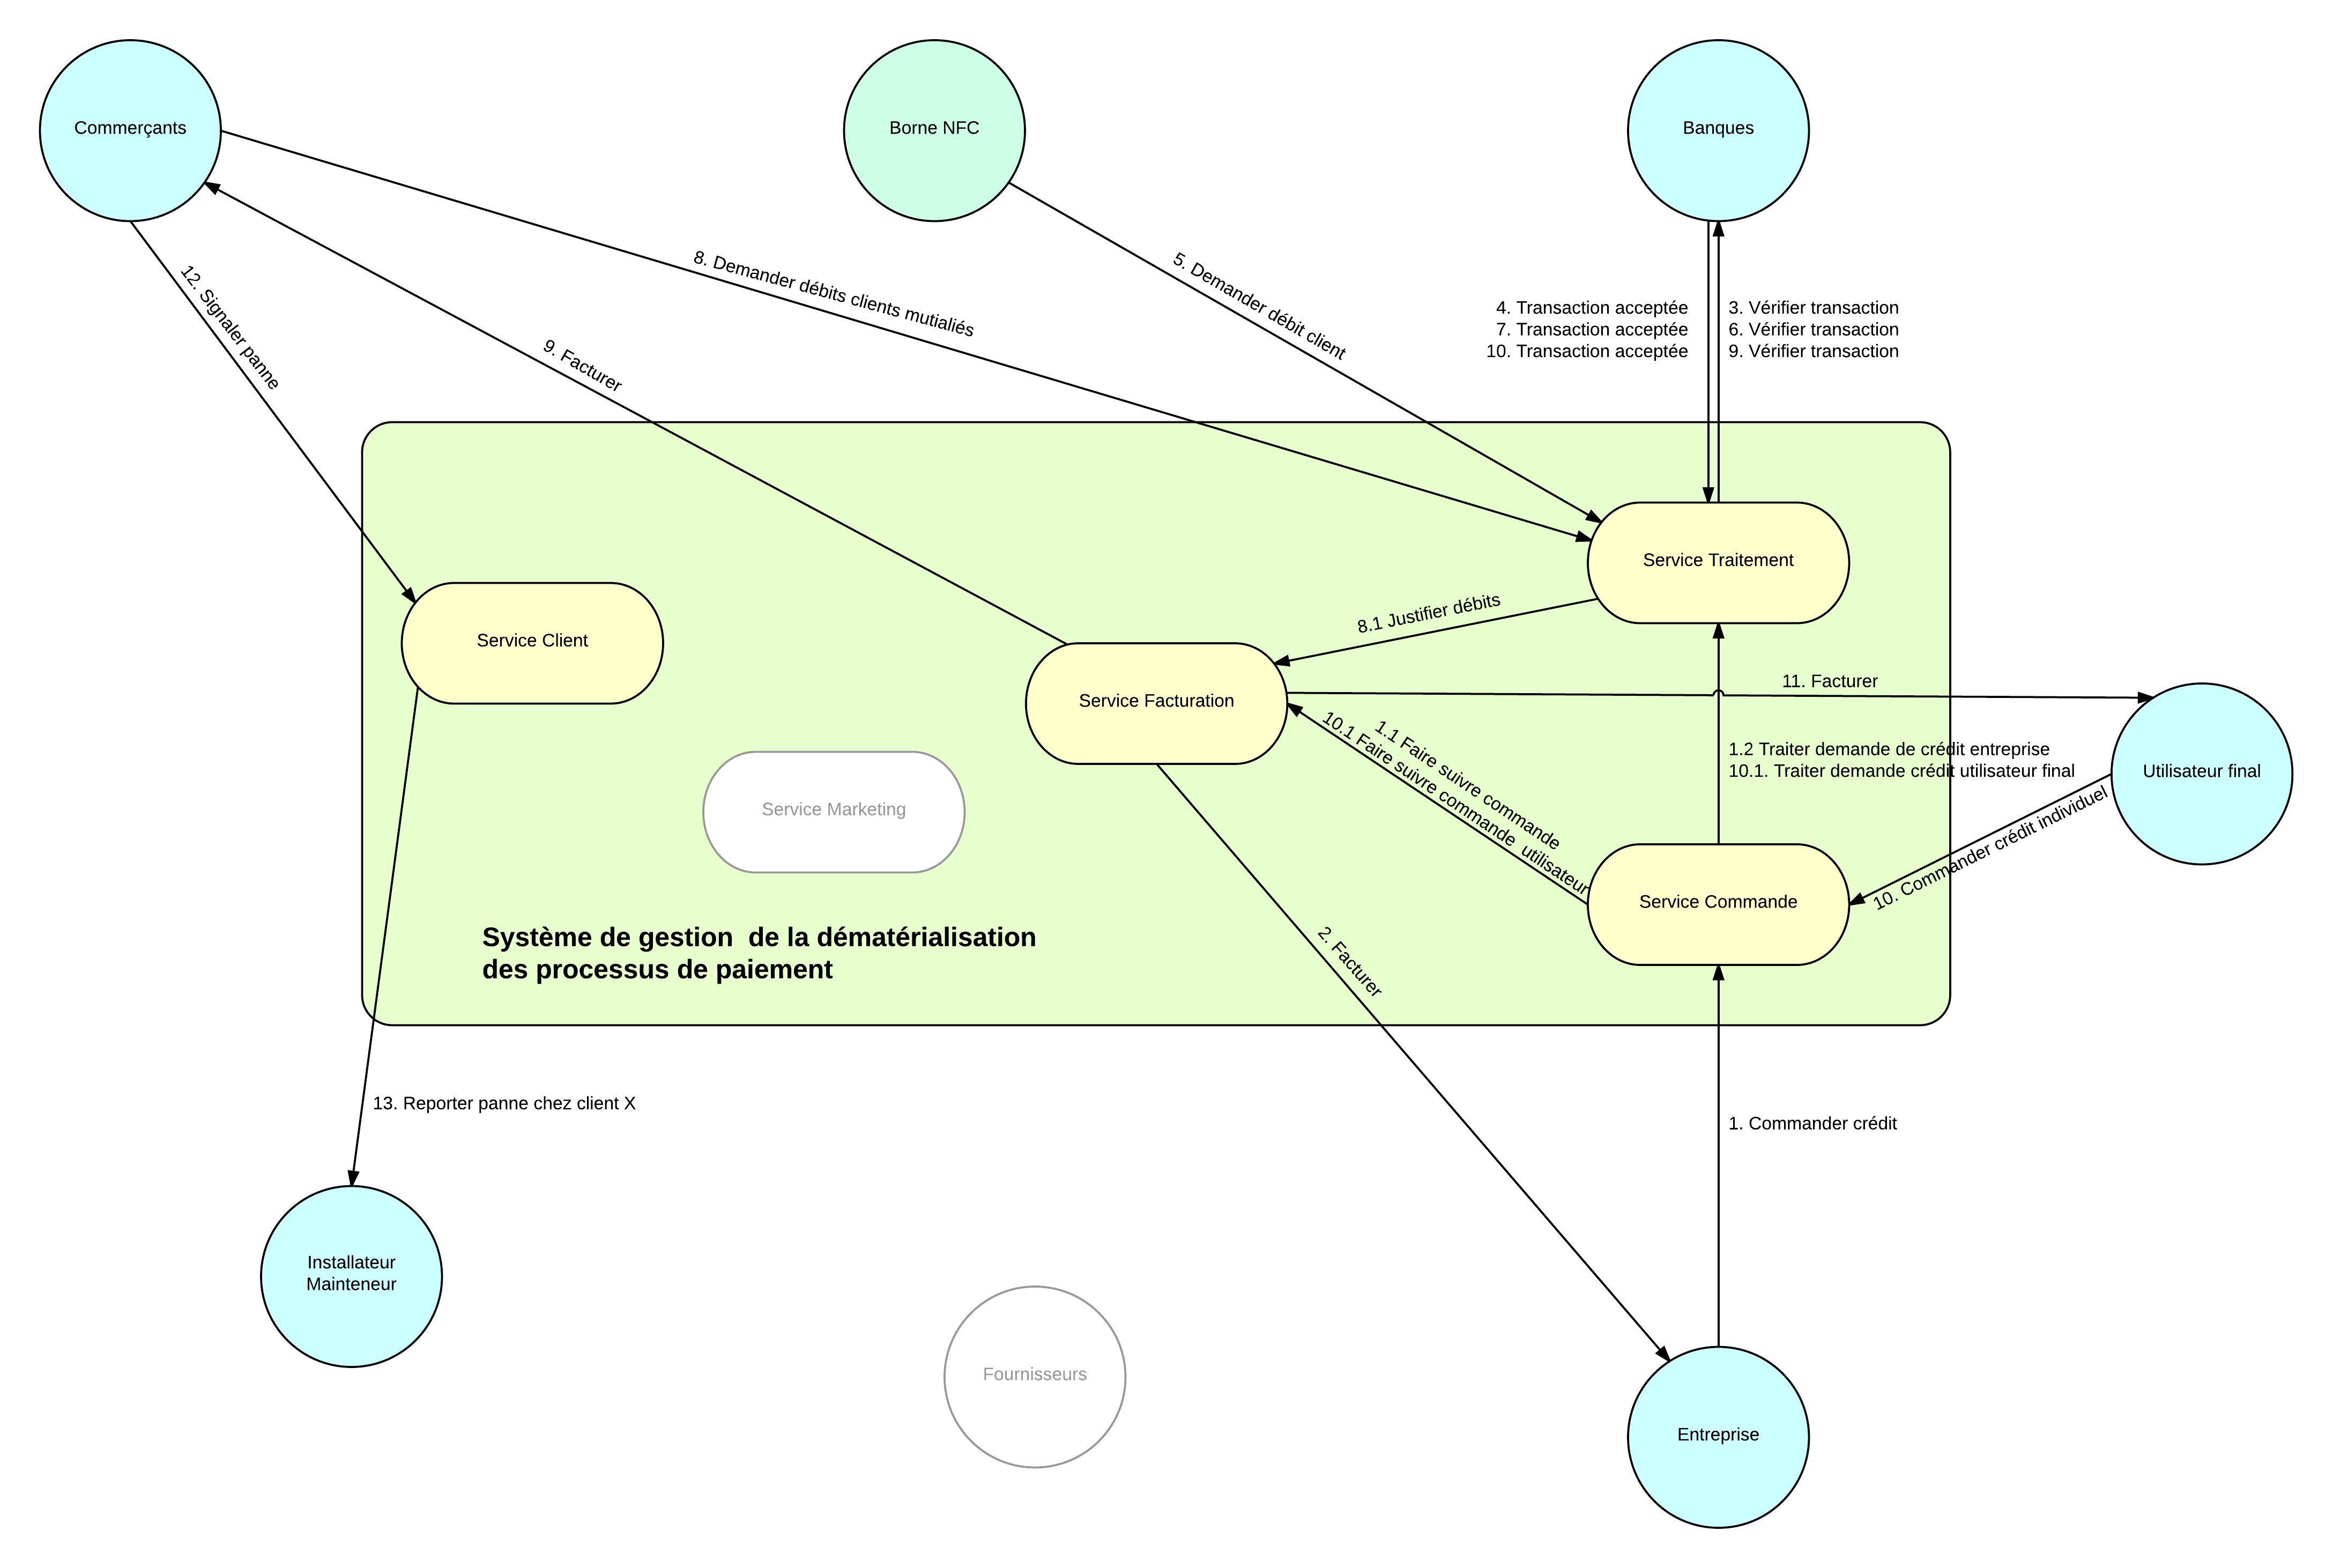
\includegraphics[width=0.7\paperheight]{mcc-extra}
      \caption{MCC Général}
      \label{fig:mcc-extra}
  \end{figure}
\end{landscape}
\newpage

\subsection{Attentes de gestion}

\subsubsection{Approvisionnement de cartes à puce}
\begin{figure}[ht]
    \centering
    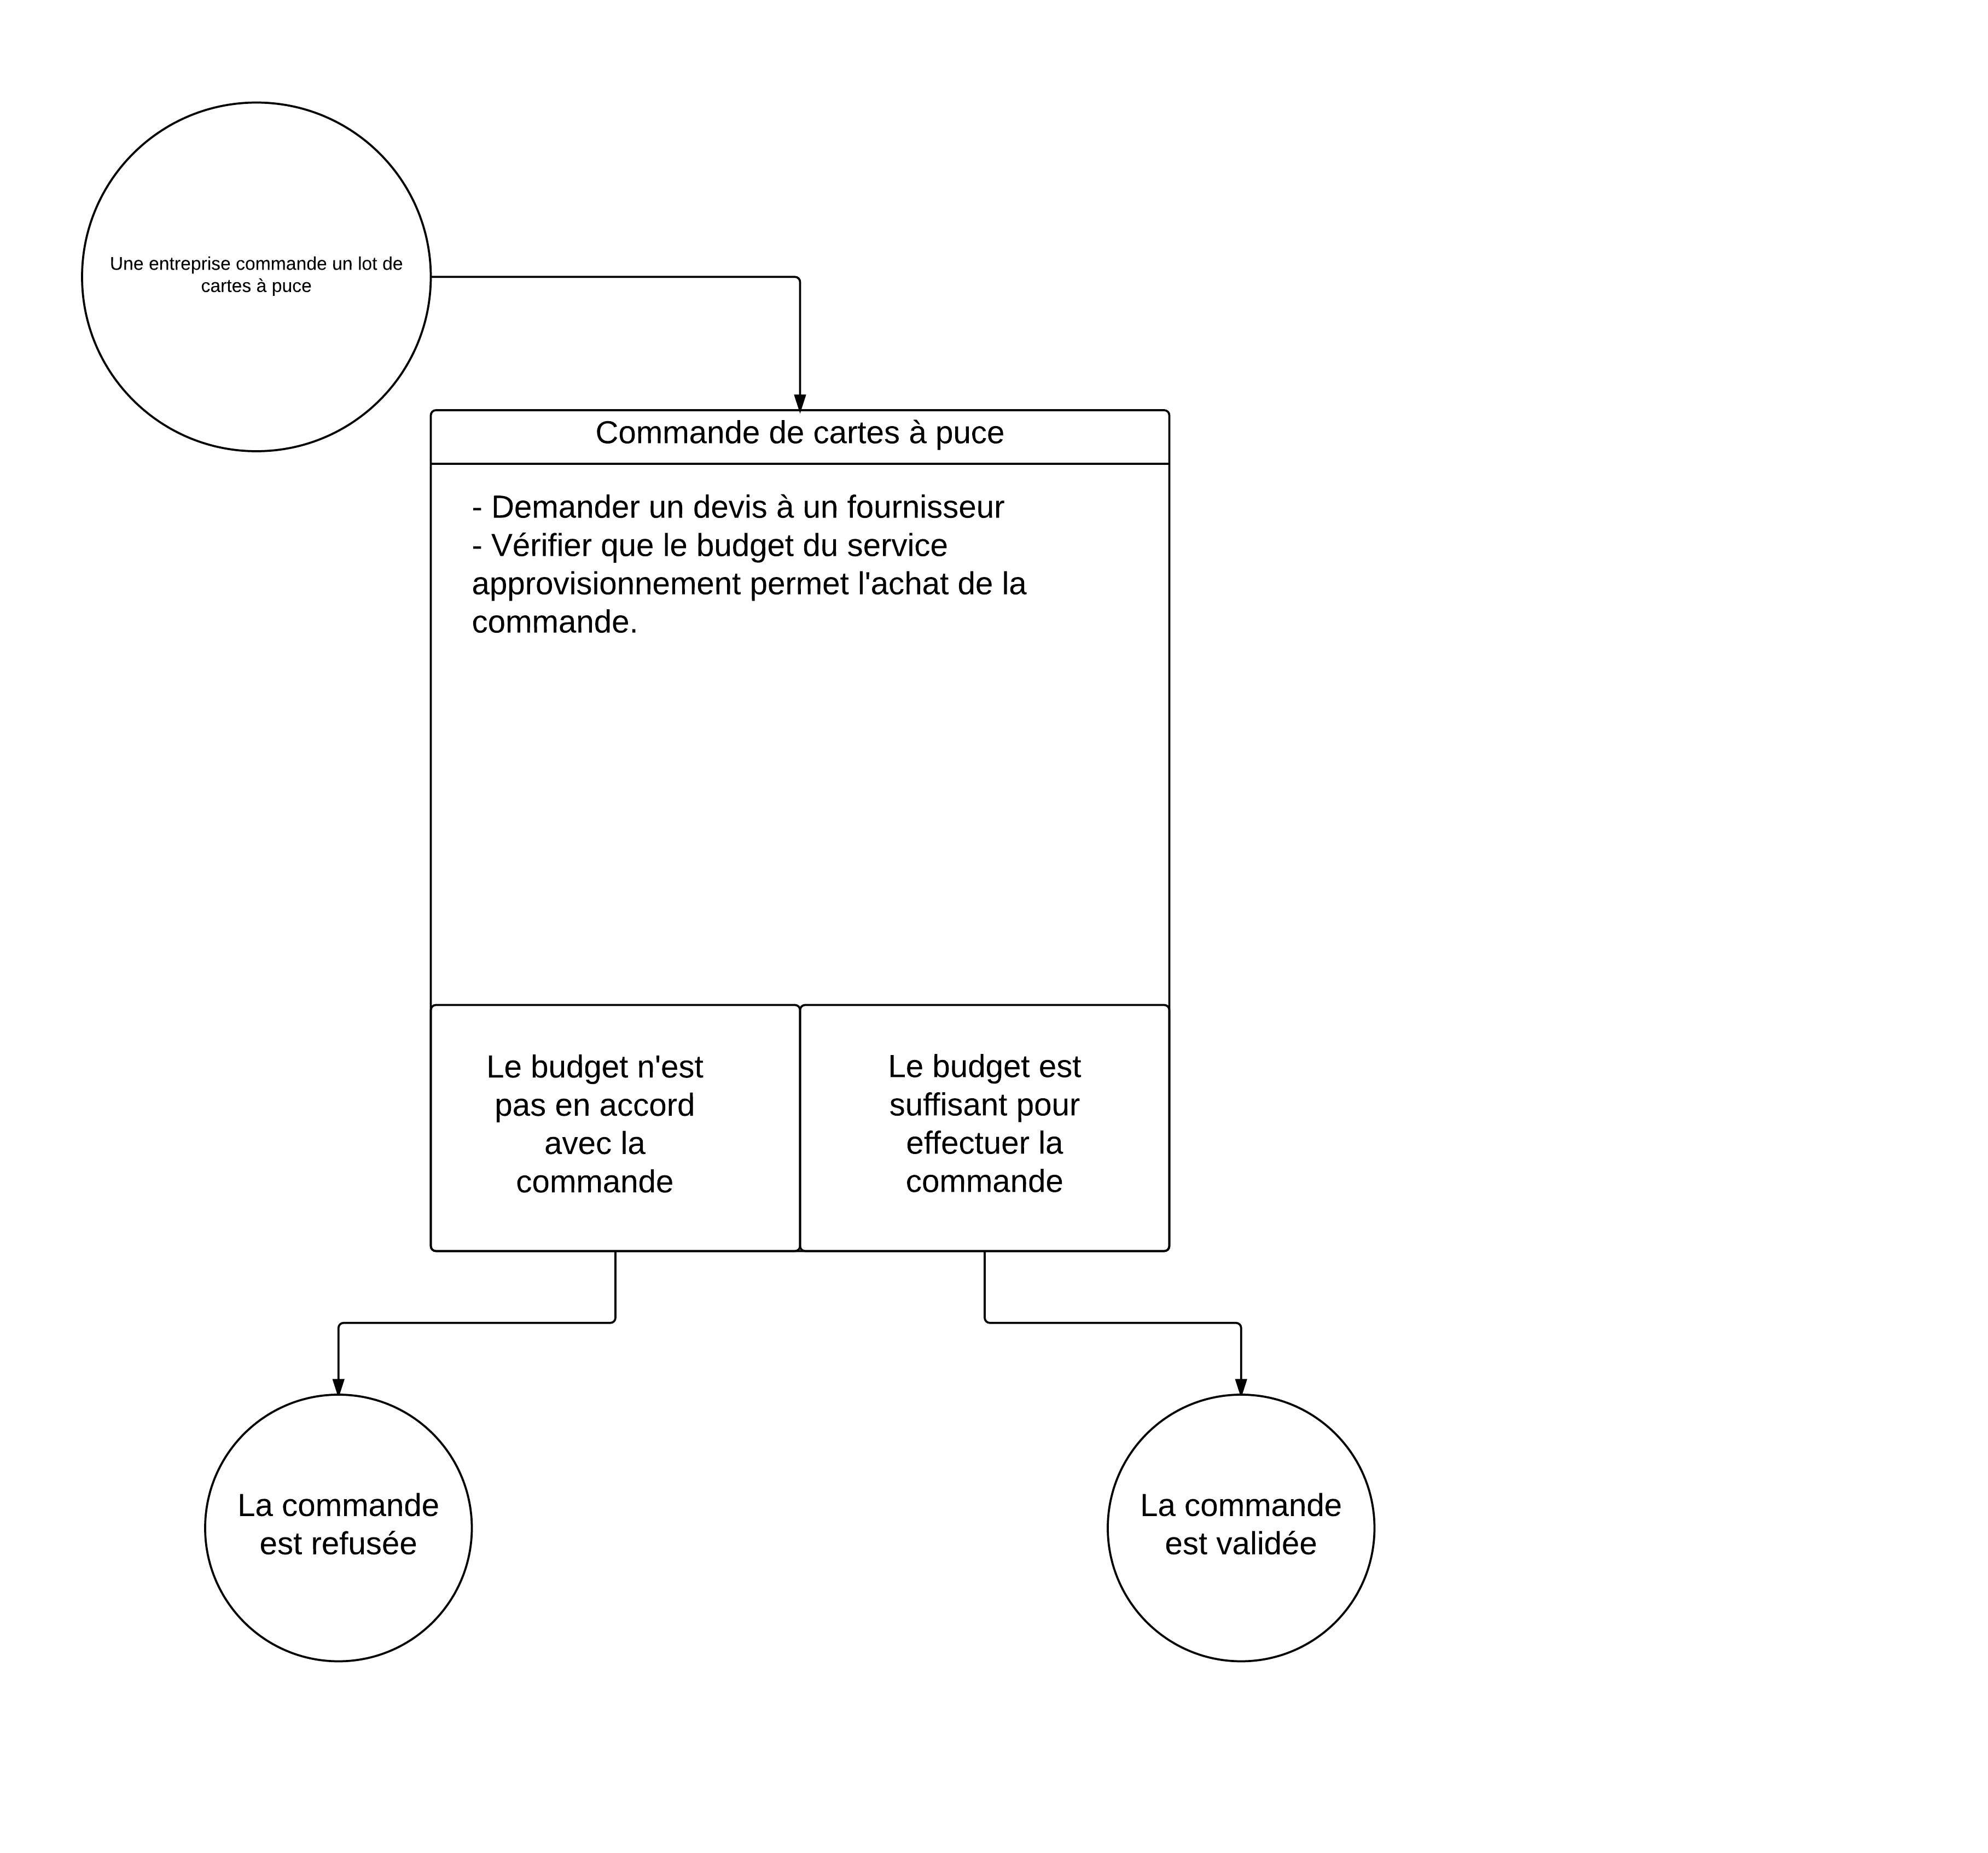
\includegraphics[width=\textwidth]{mot-approvisionnement-cartes-a-puce}
    \caption{MOT : Approvisionnement des cartes à puce}
    \label{fig:mot-approvisionnement-cartes-a-puce}
\end{figure}
\newpage

\subsubsection{Éditer une facture pour une commande}
\begin{figure}[ht]
    \centering
    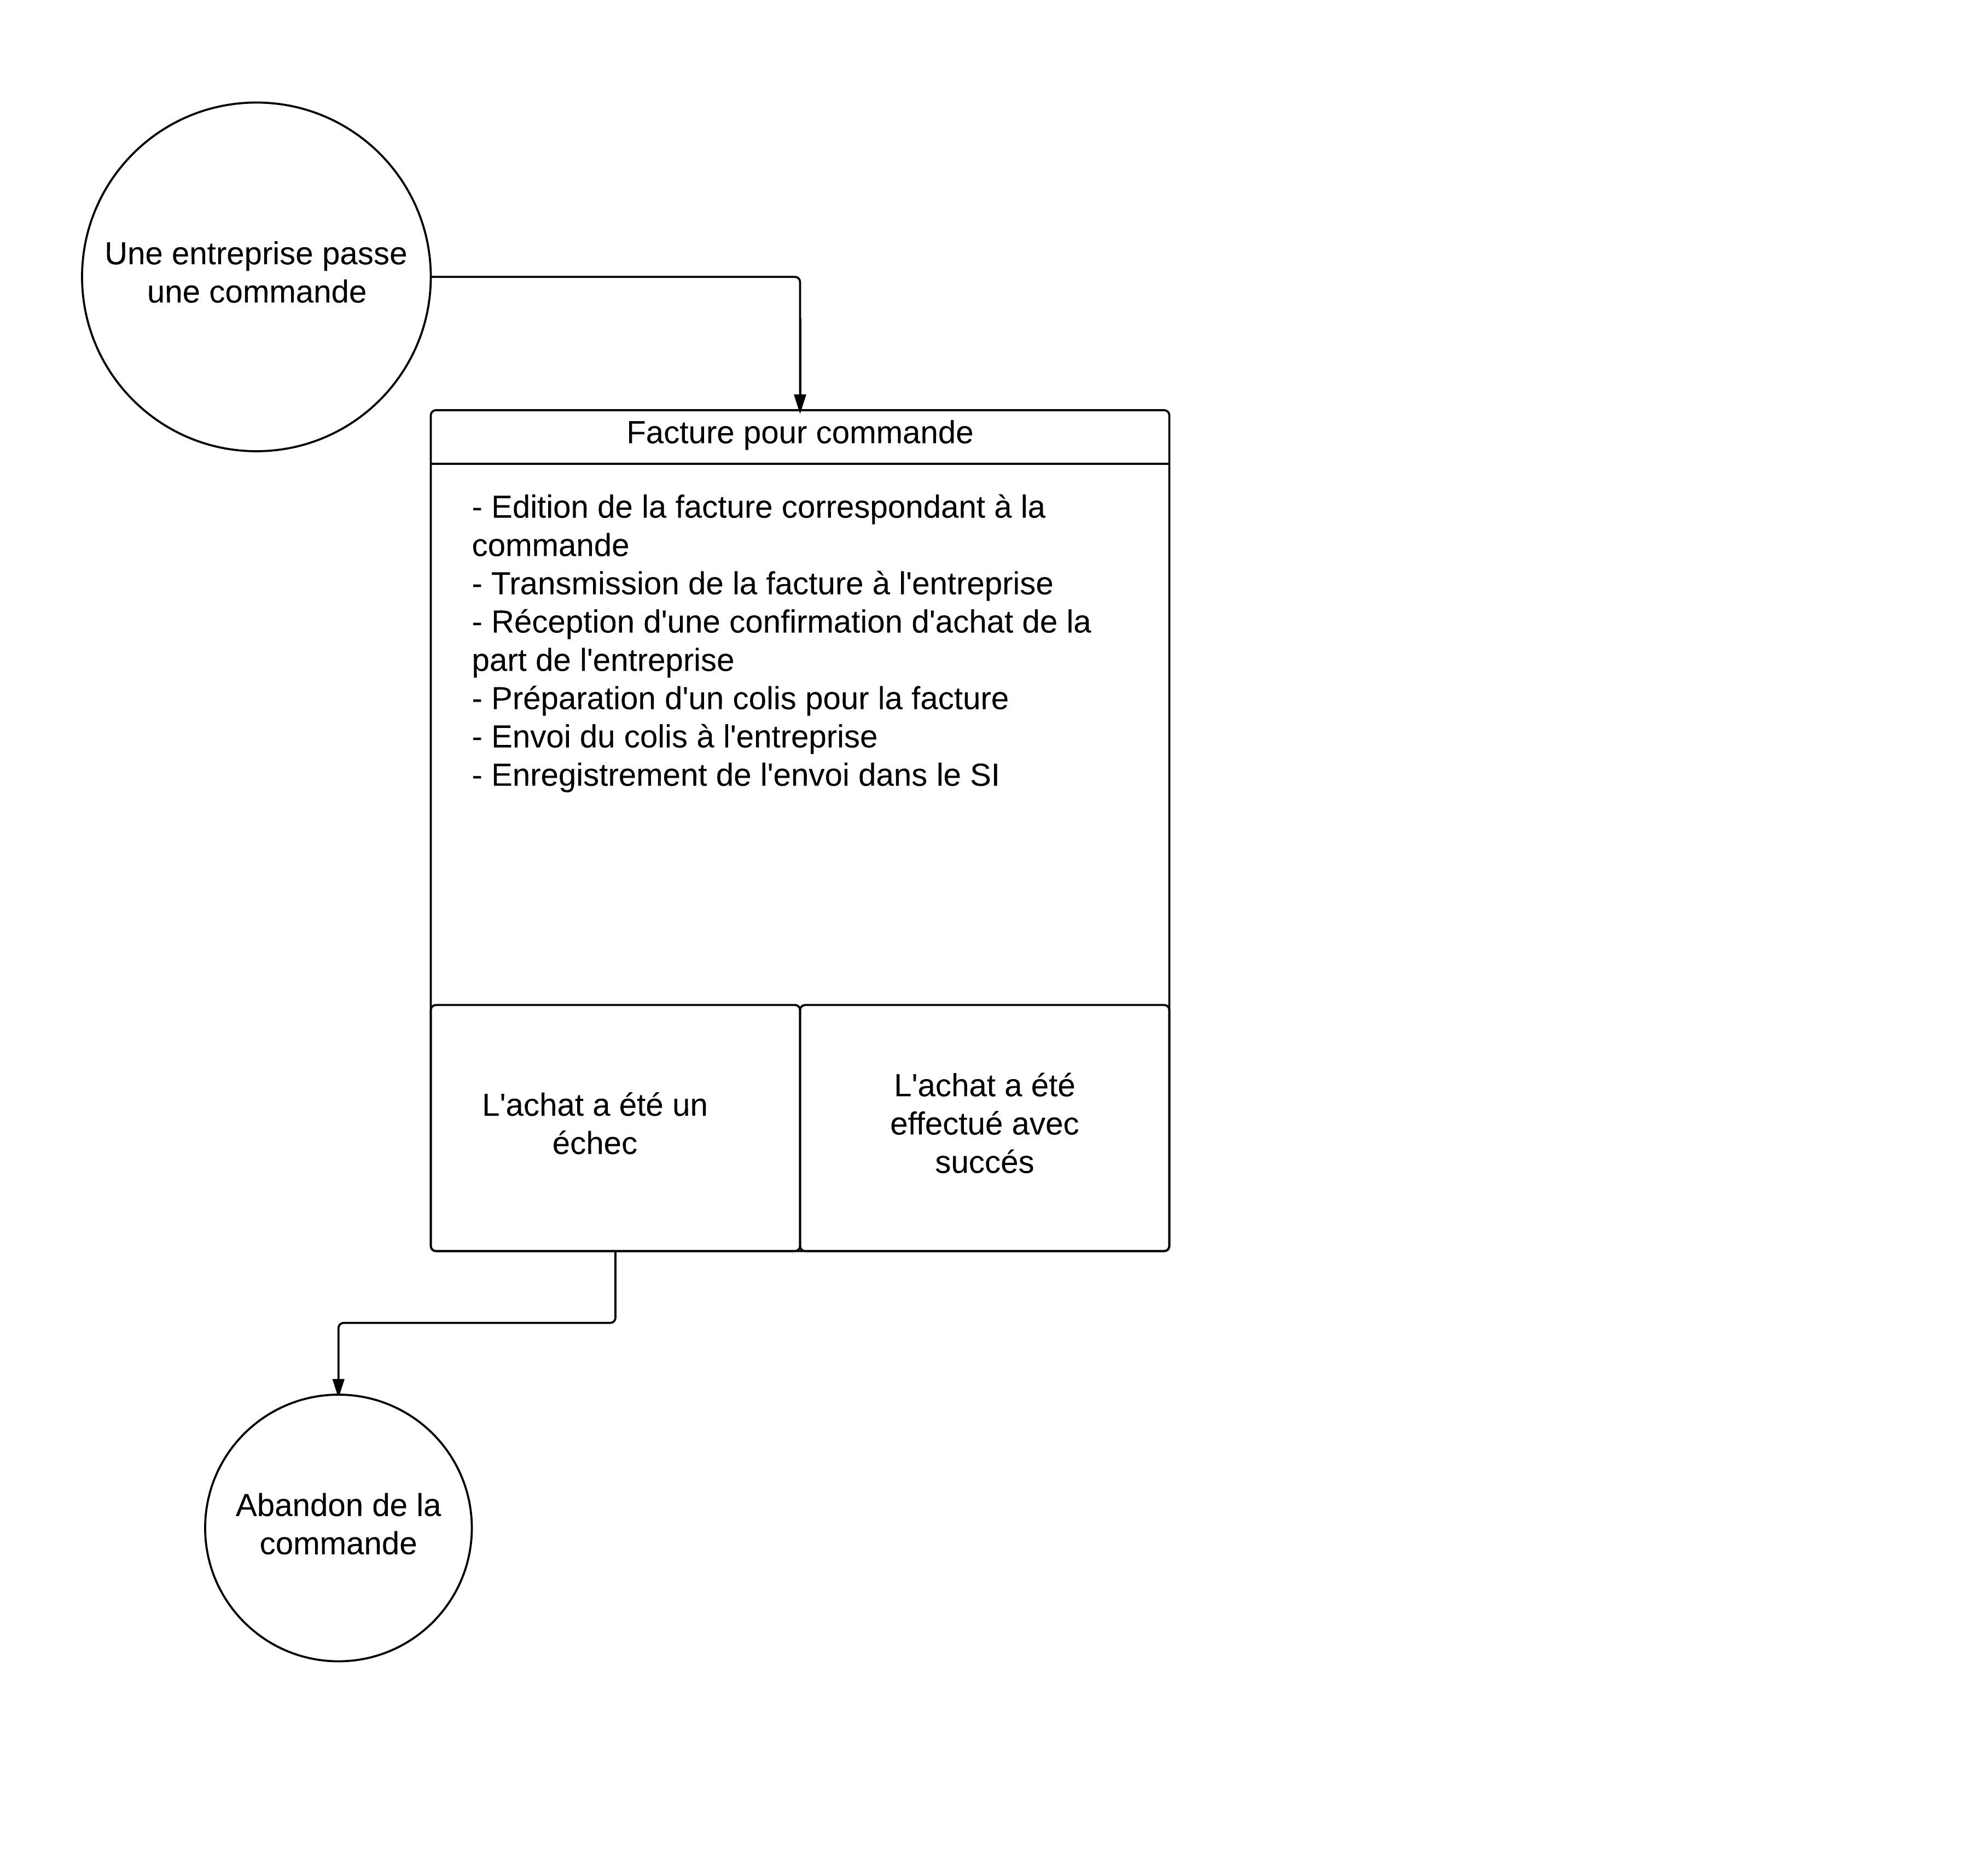
\includegraphics[width=\textwidth]{mot-editer-facture-commande}
    \caption{MOT : Editer d'une facture pour une commande}
    \label{fig:mot-editer-facture-commande}
\end{figure}
\newpage

\subsubsection{Effectuer une commande de cartes à puce}
\begin{figure}[ht]
    \centering
    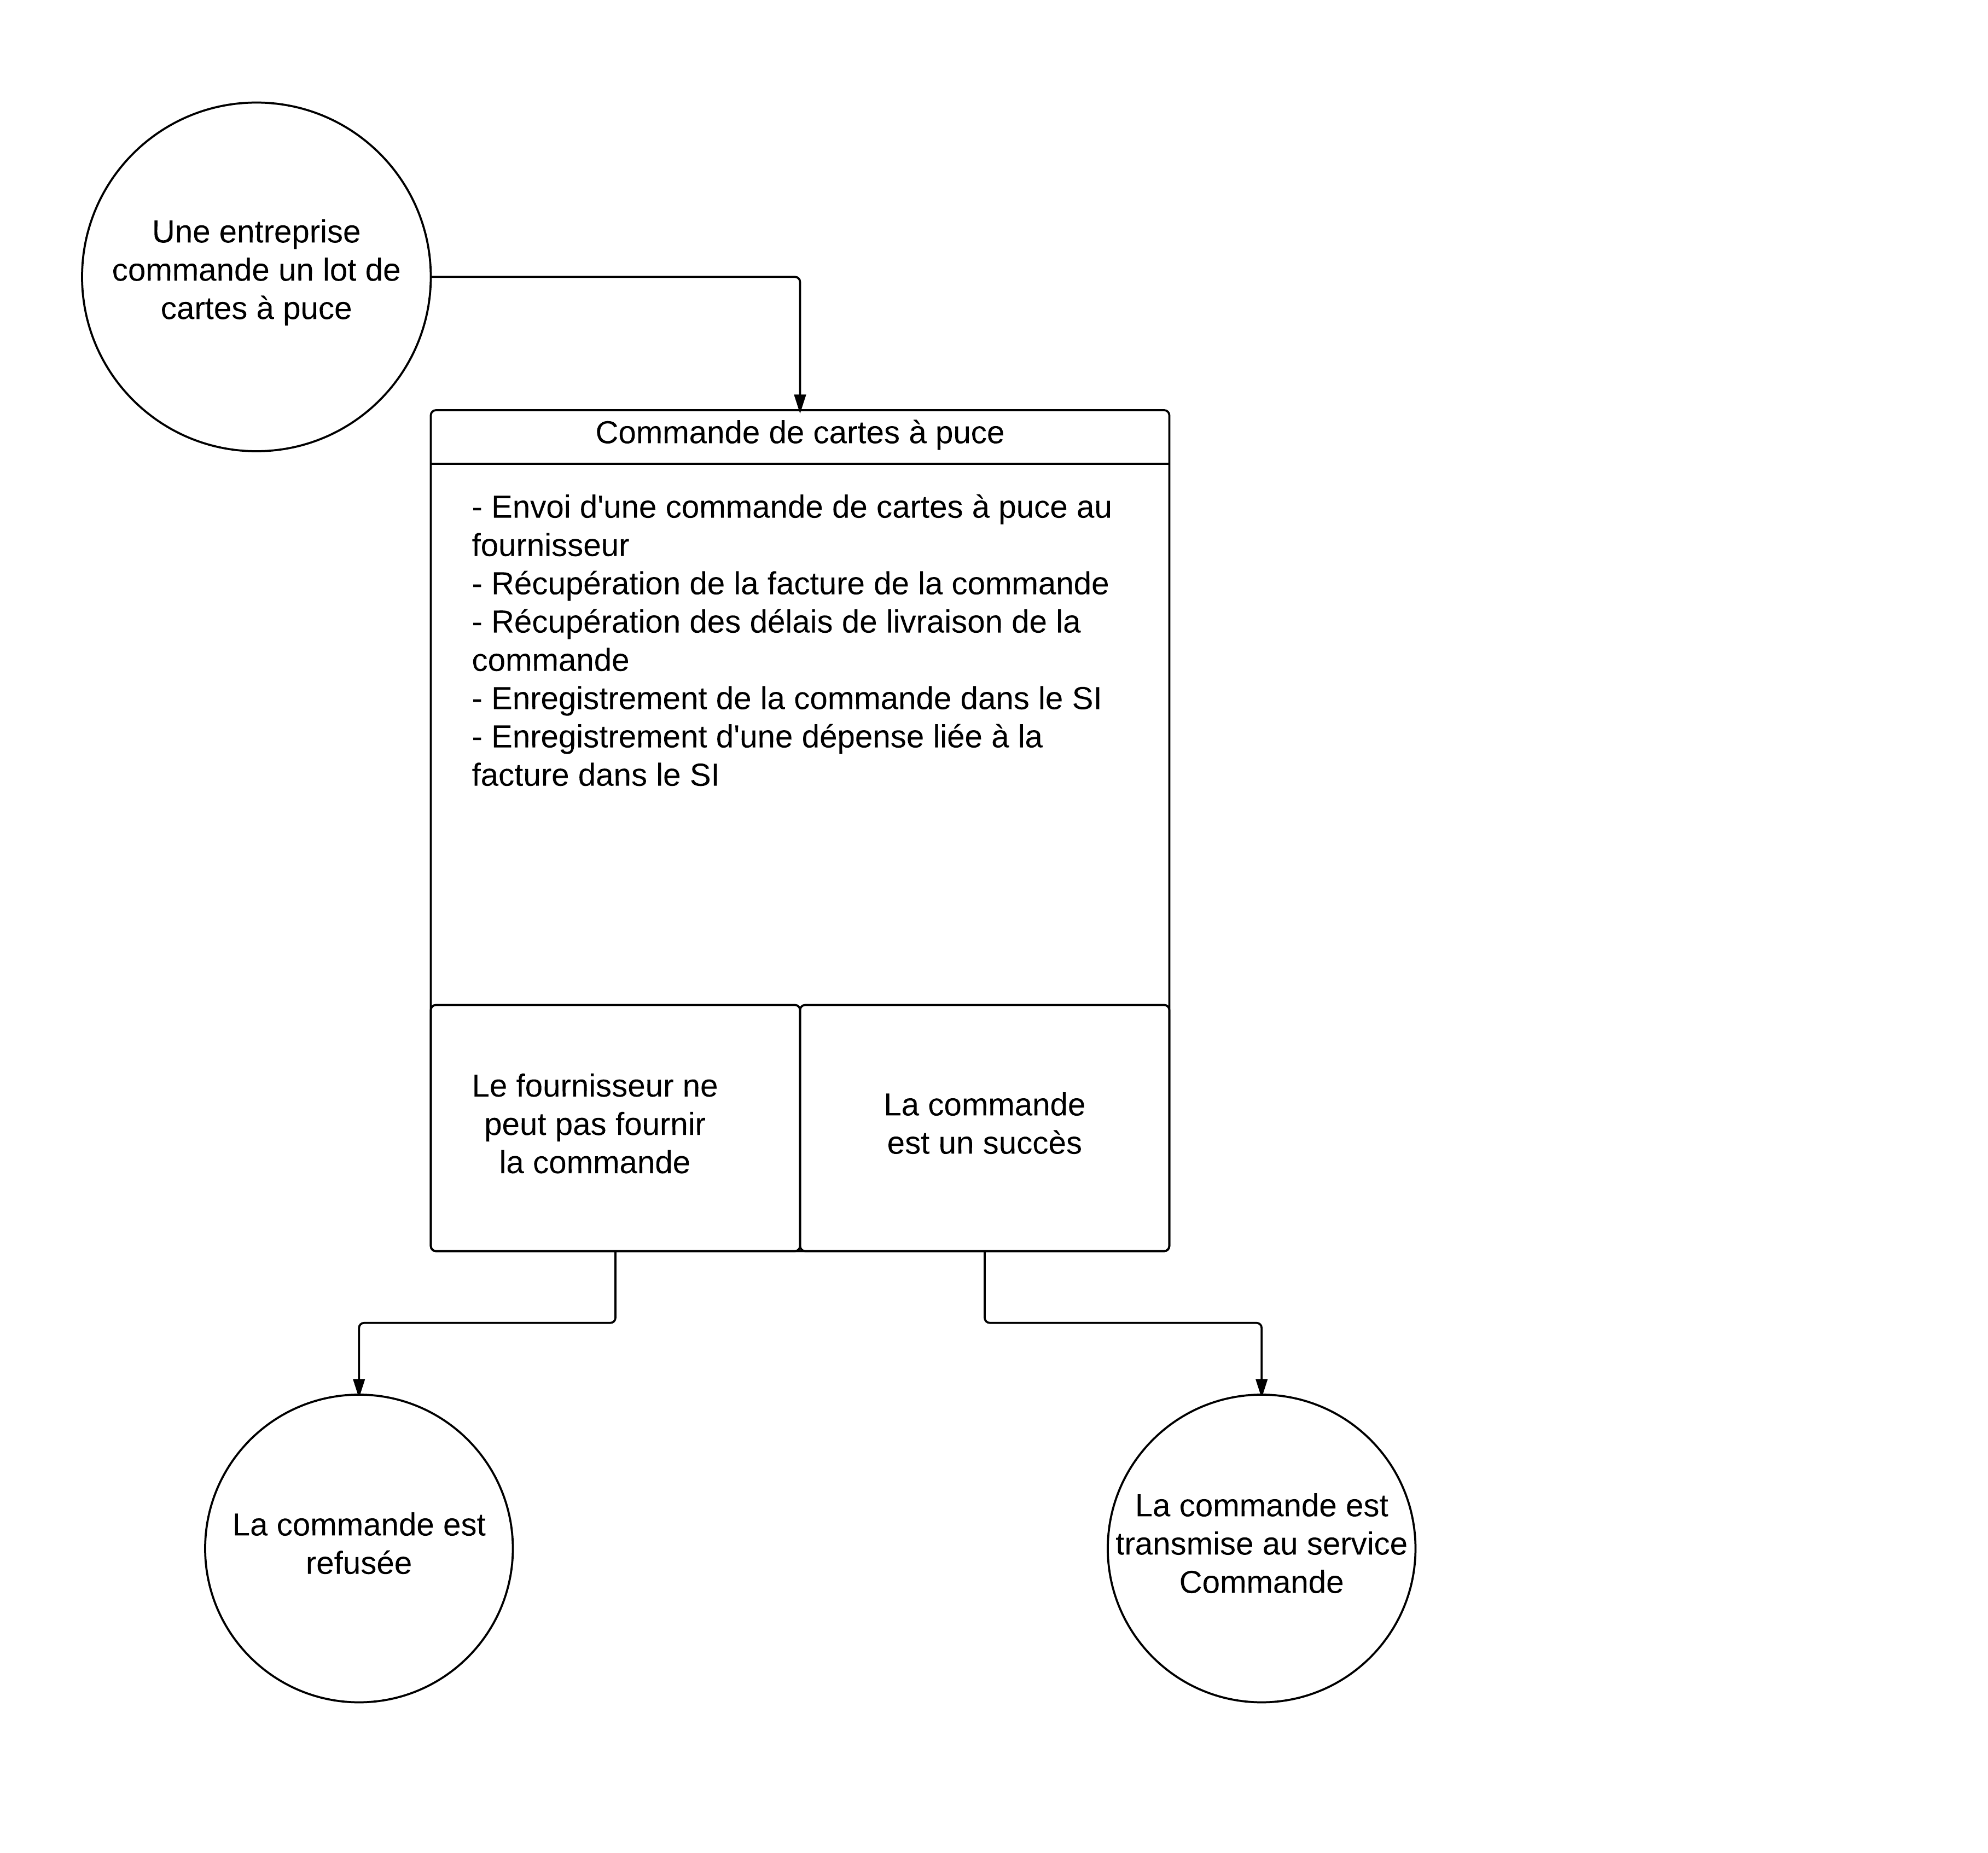
\includegraphics[width=\textwidth]{mot-effectuer-commande-cartes-a-puce}
    \caption{MOT : Effectuer une commande de cartes à puce}
    \label{fig:mot-effectuer-commande-cartes-a-puce}
\end{figure}
\newpage

\subsubsection{Inscription d'une entreprise}
\begin{figure}[ht]
    \centering
    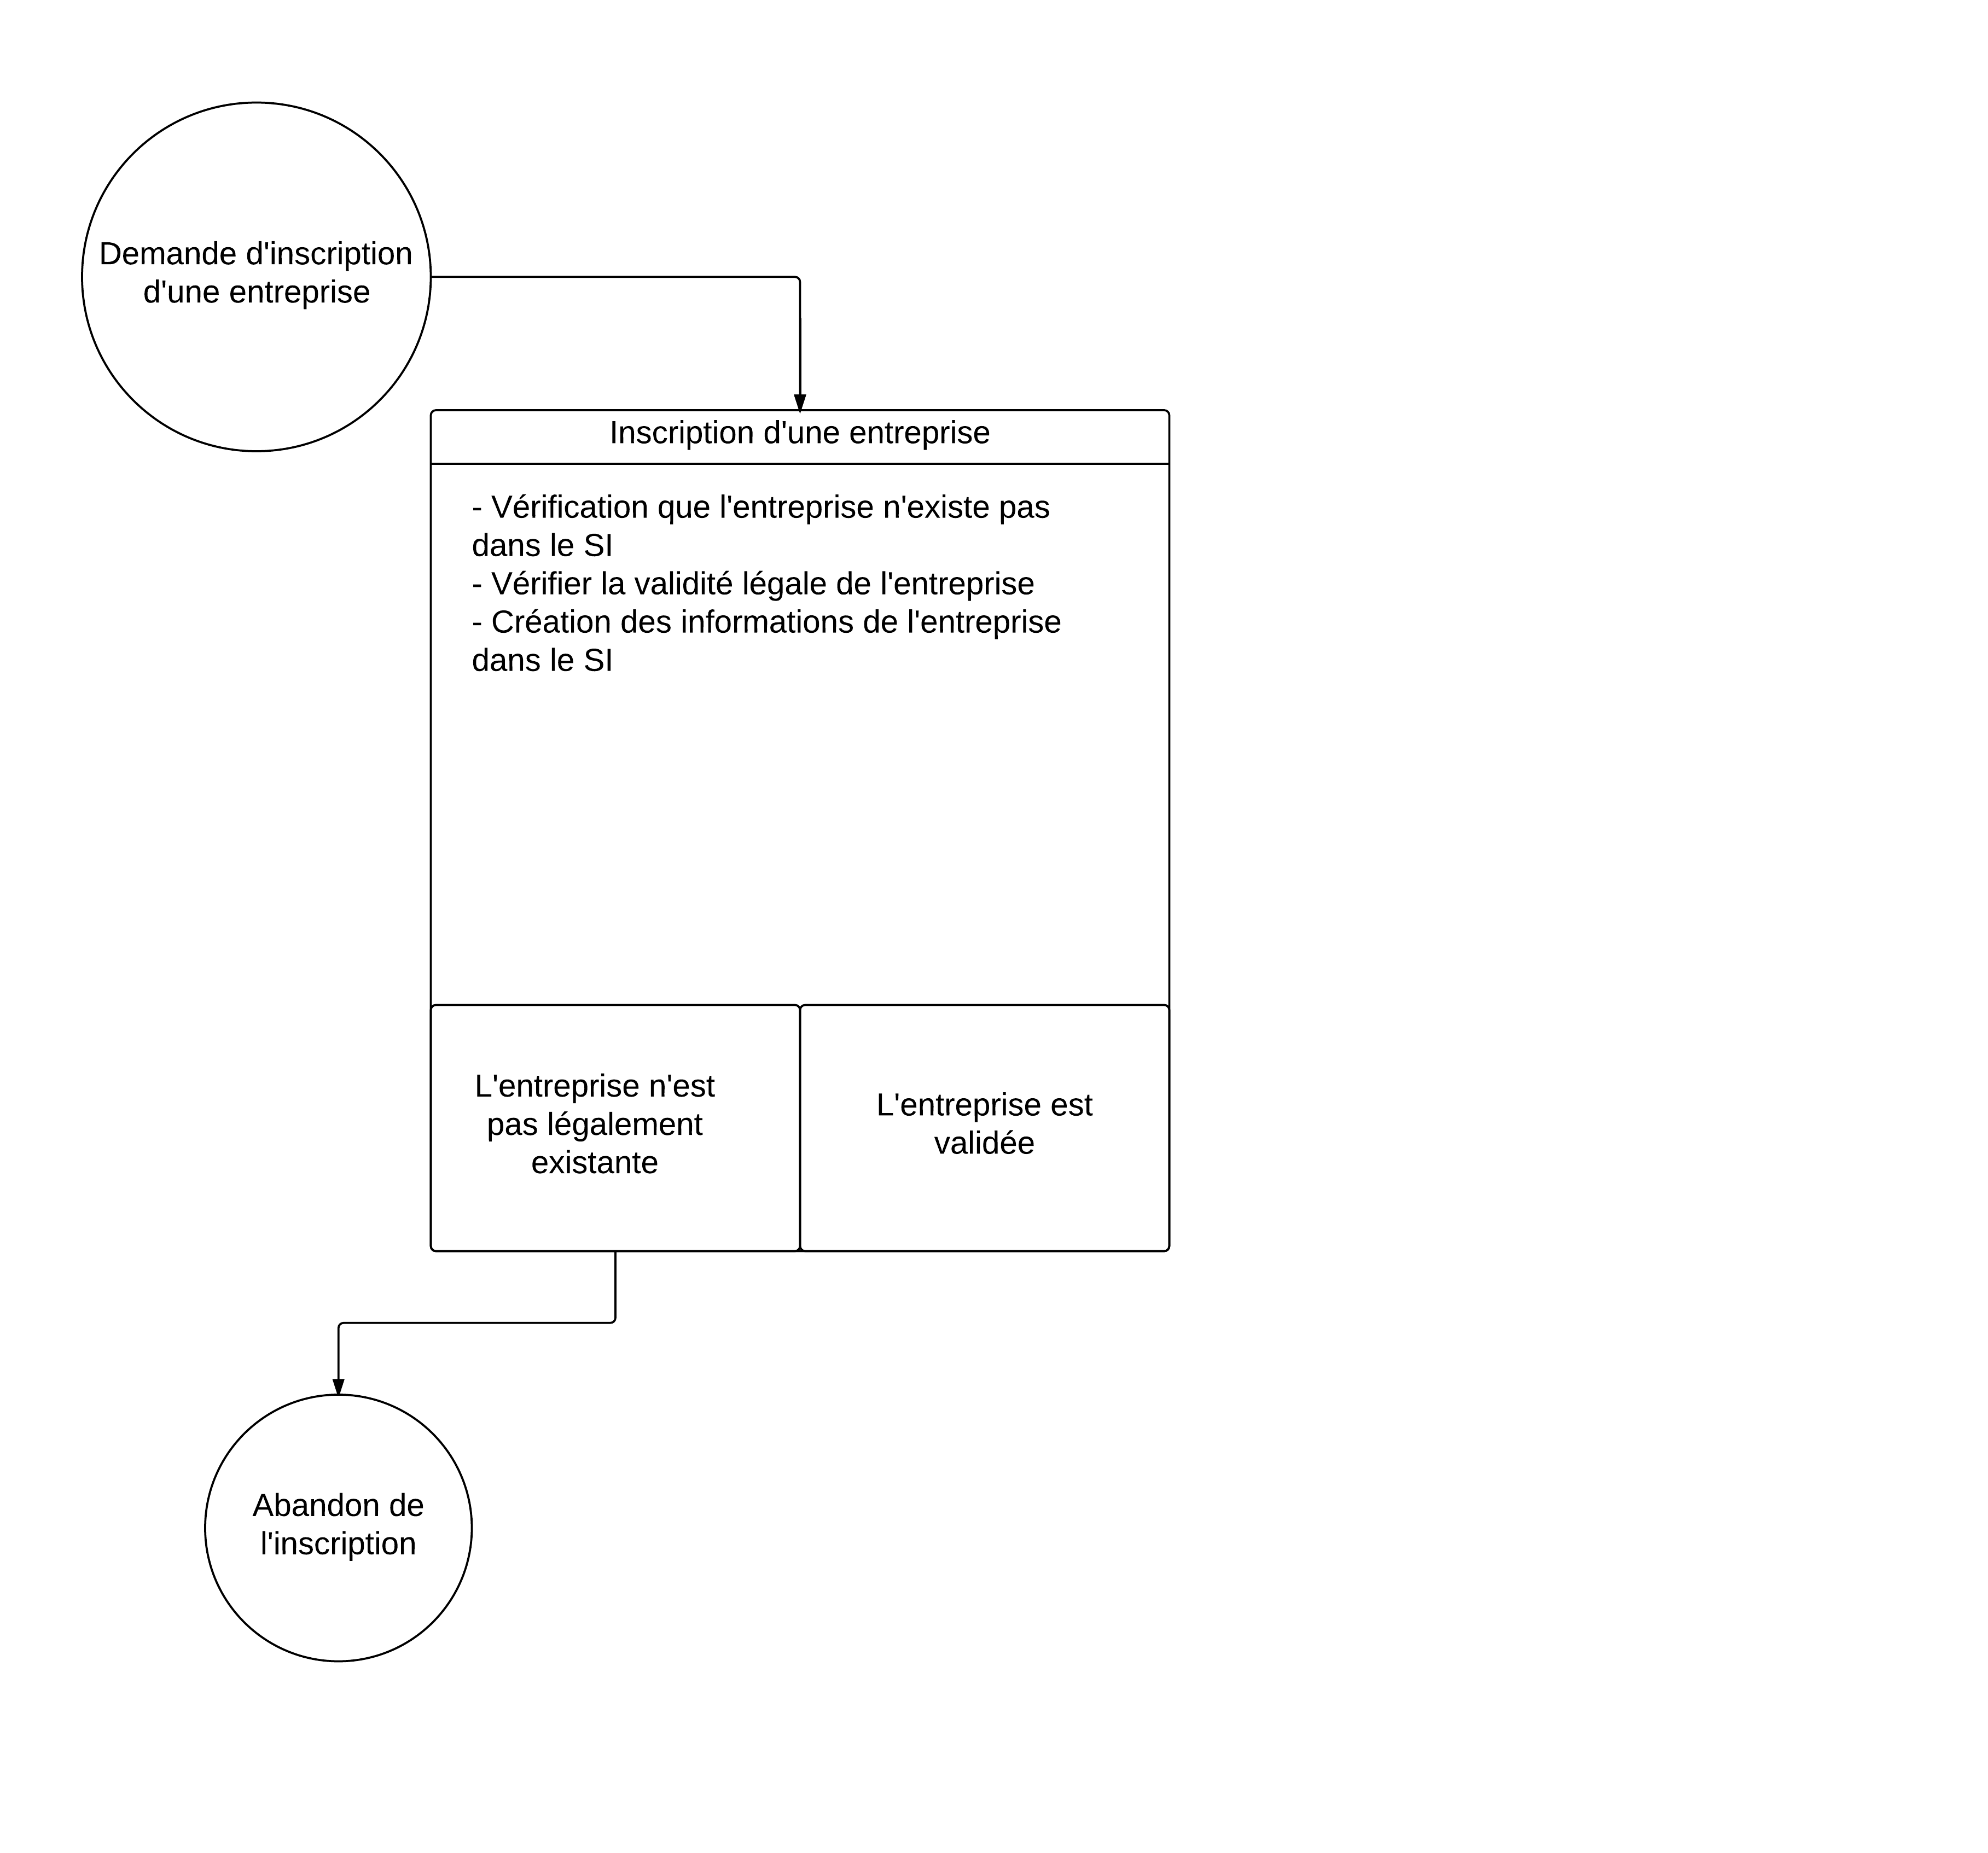
\includegraphics[width=\textwidth]{mot-inscription-entreprise}
    \caption{MOT : Inscription d'une entreprise}
    \label{fig:mot-inscription-entreprise}
\end{figure}
\newpage

\subsubsection{Traitement des commandes}
\begin{figure}[ht]
    \centering
    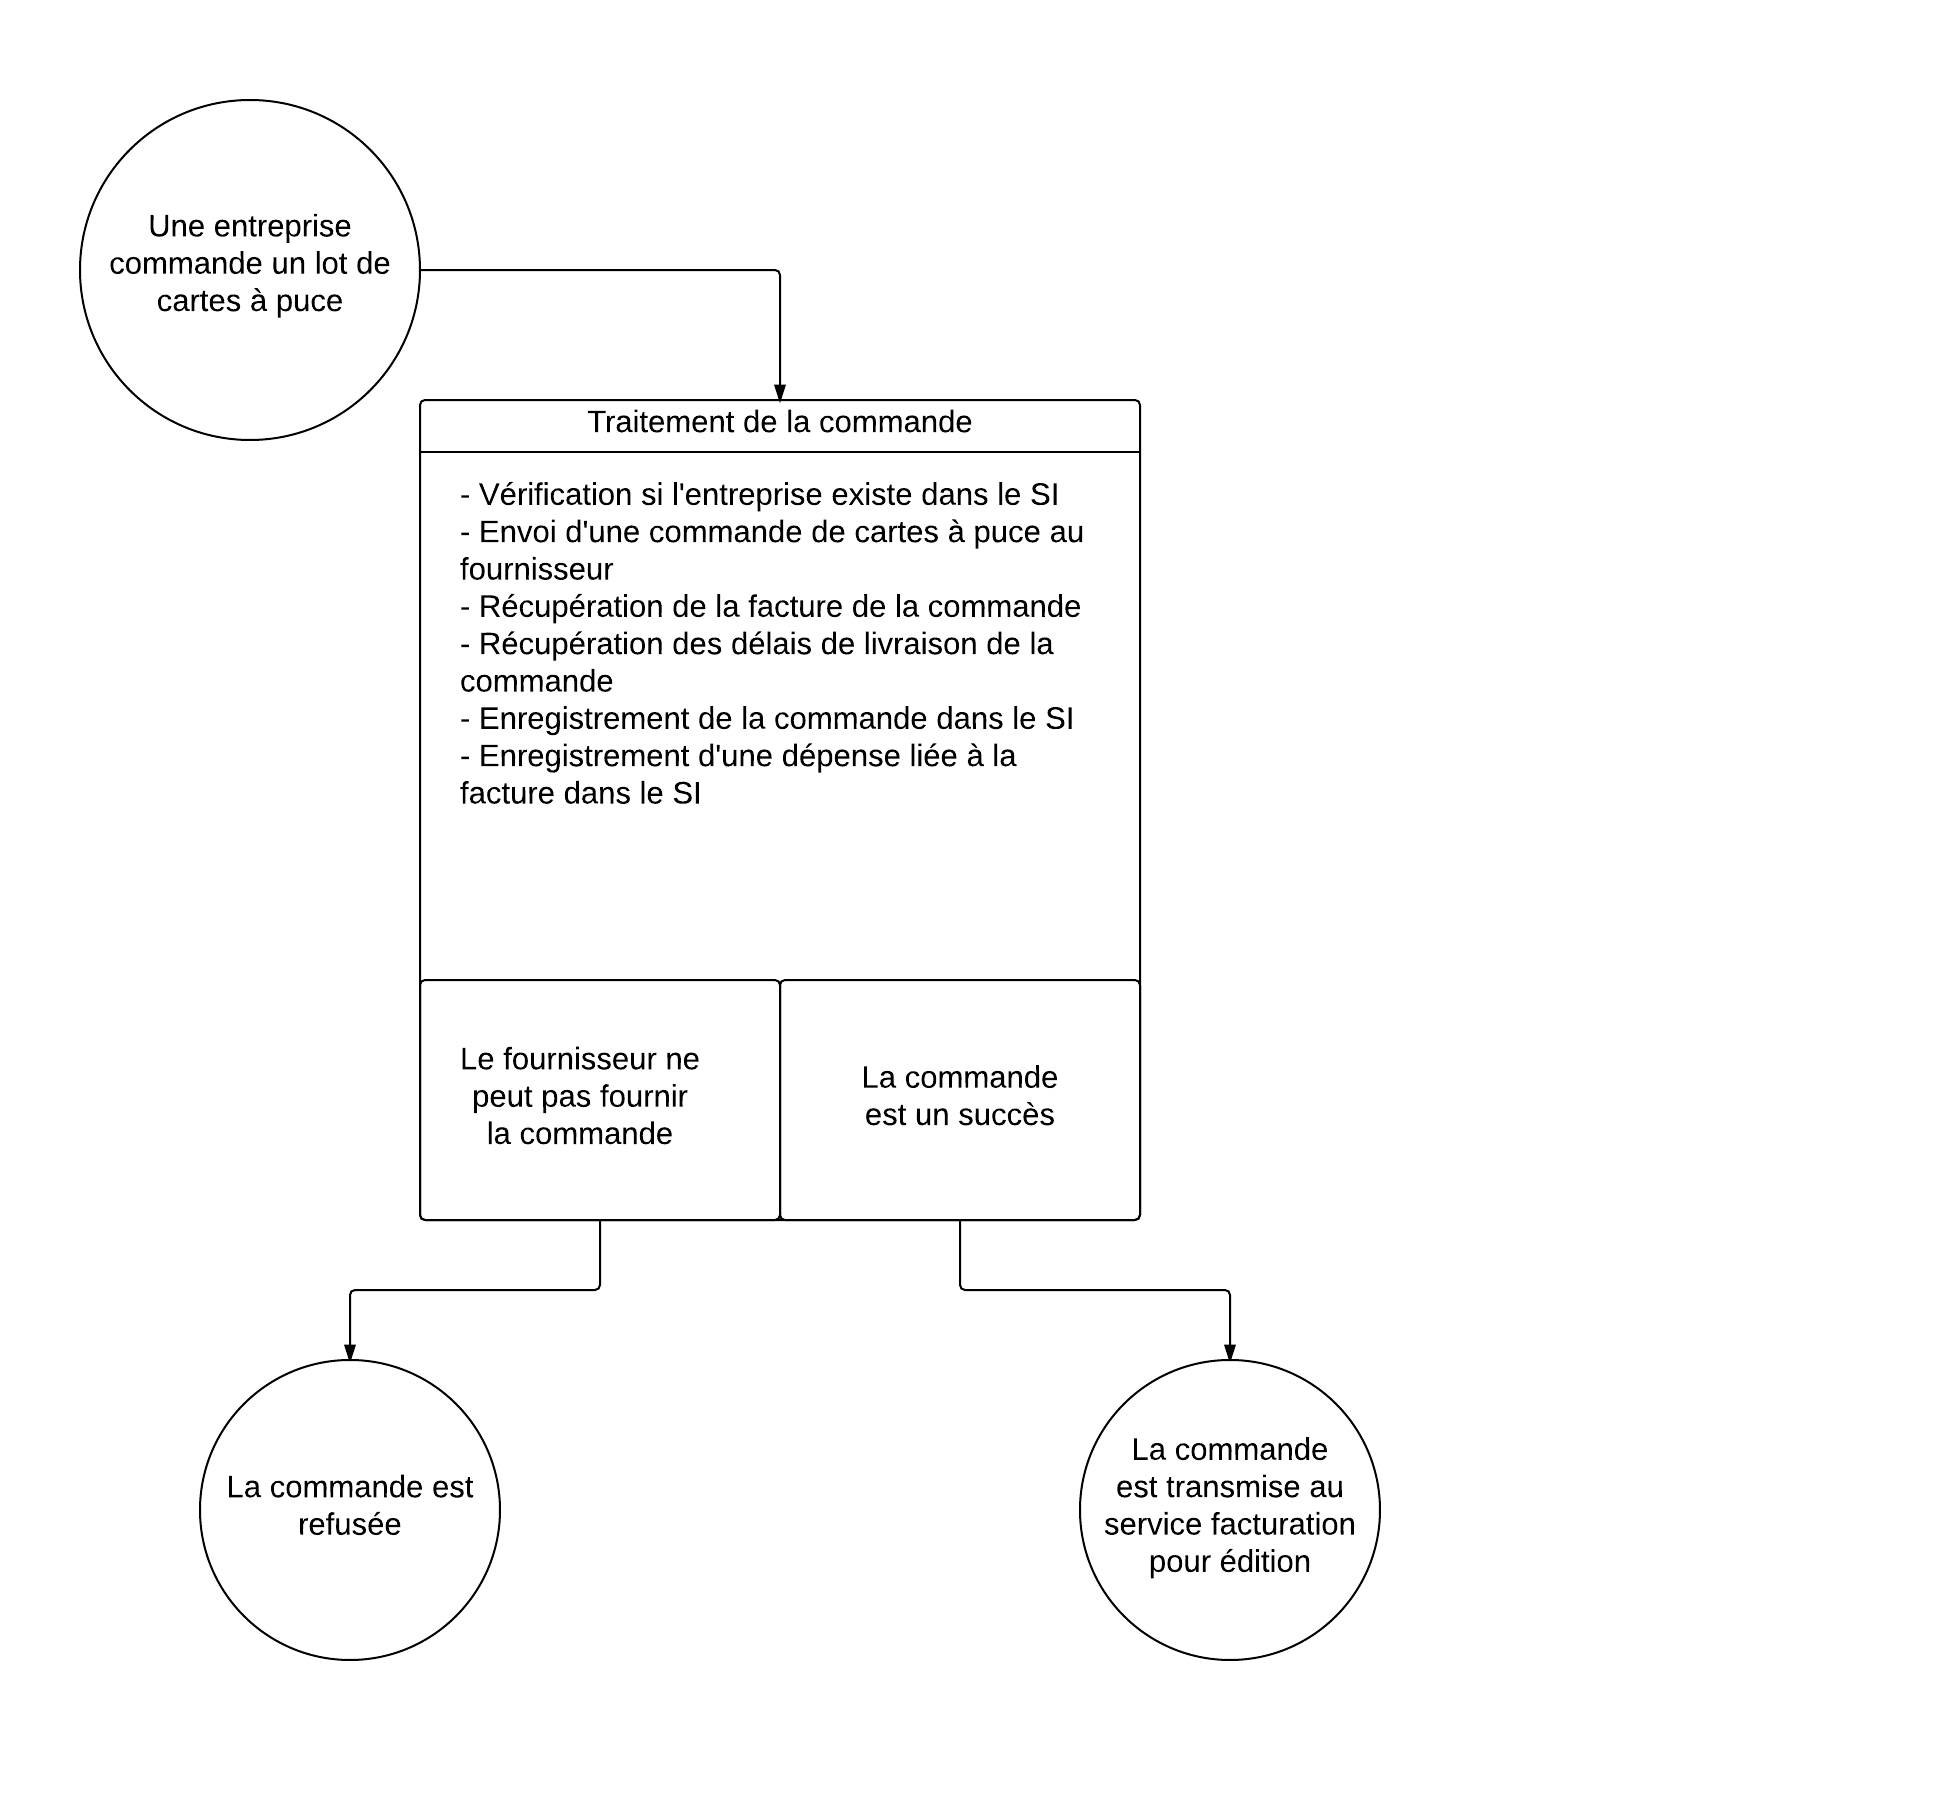
\includegraphics[width=\textwidth]{mot-traitement-commandes}
    \caption{MOT : Traitement des commandes}
    \label{fig:mot-traitement-commandes}
\end{figure}
\newpage

\subsubsection{Demande de devis d'approvisionnement}

La demande de devis d'approvisionnement se fait entièrement par le service
approvisionnement. \\

La demande de devis d'approvisionnement devra se faire par un premier
contact avec un fournisseur de cartes à puce. Bien évidemment, on
envisagera de changer de fournisseur en cas de dégradation du service ou
d'augmentation des prix. Au contraire, après premier contact et si le
fournisseur actuel offre un rabais conséquent sur commande, on gardera contact
avec ce dernier pour les commandes suivantes. \\

Après réception du devis indiquant les modalités de livraison telles que le
délai ou encore le prix, le service approvisionnement transmettra ces dernières
au service commande pour qu'il reprenne le traitement de la commande.

\subsubsection{Refus d'une commande}

Le refus d'une commande est effectué dans le cas où le budget attribué au
service approvisionnement est épuisé et ne peut pas être renouvelé, ou bien si
aucun fournisseur n'est en mesure de livrer une commande de cartes à puce. \\

Le service commande informe par la suite l'entreprise ayant saisie la commande
pour lui indiquer que la commande ne pourra pas être effectuée. Il faut noter
que ce cas est très rare et ne devait normalement pas apparaître vu qu'il
suppose qu'\textbf{aucun fournisseur n'est disponible}. Le service commande
devra insister sur ce dernier point afin de conserver une image correcte auprès
de l'entreprise.

\subsection{Attentes métier}
\subsection{Attentes B2B/B2C}

\subsubsection{Prospection des clients}

\begin{figure}[ht]
    \centering
    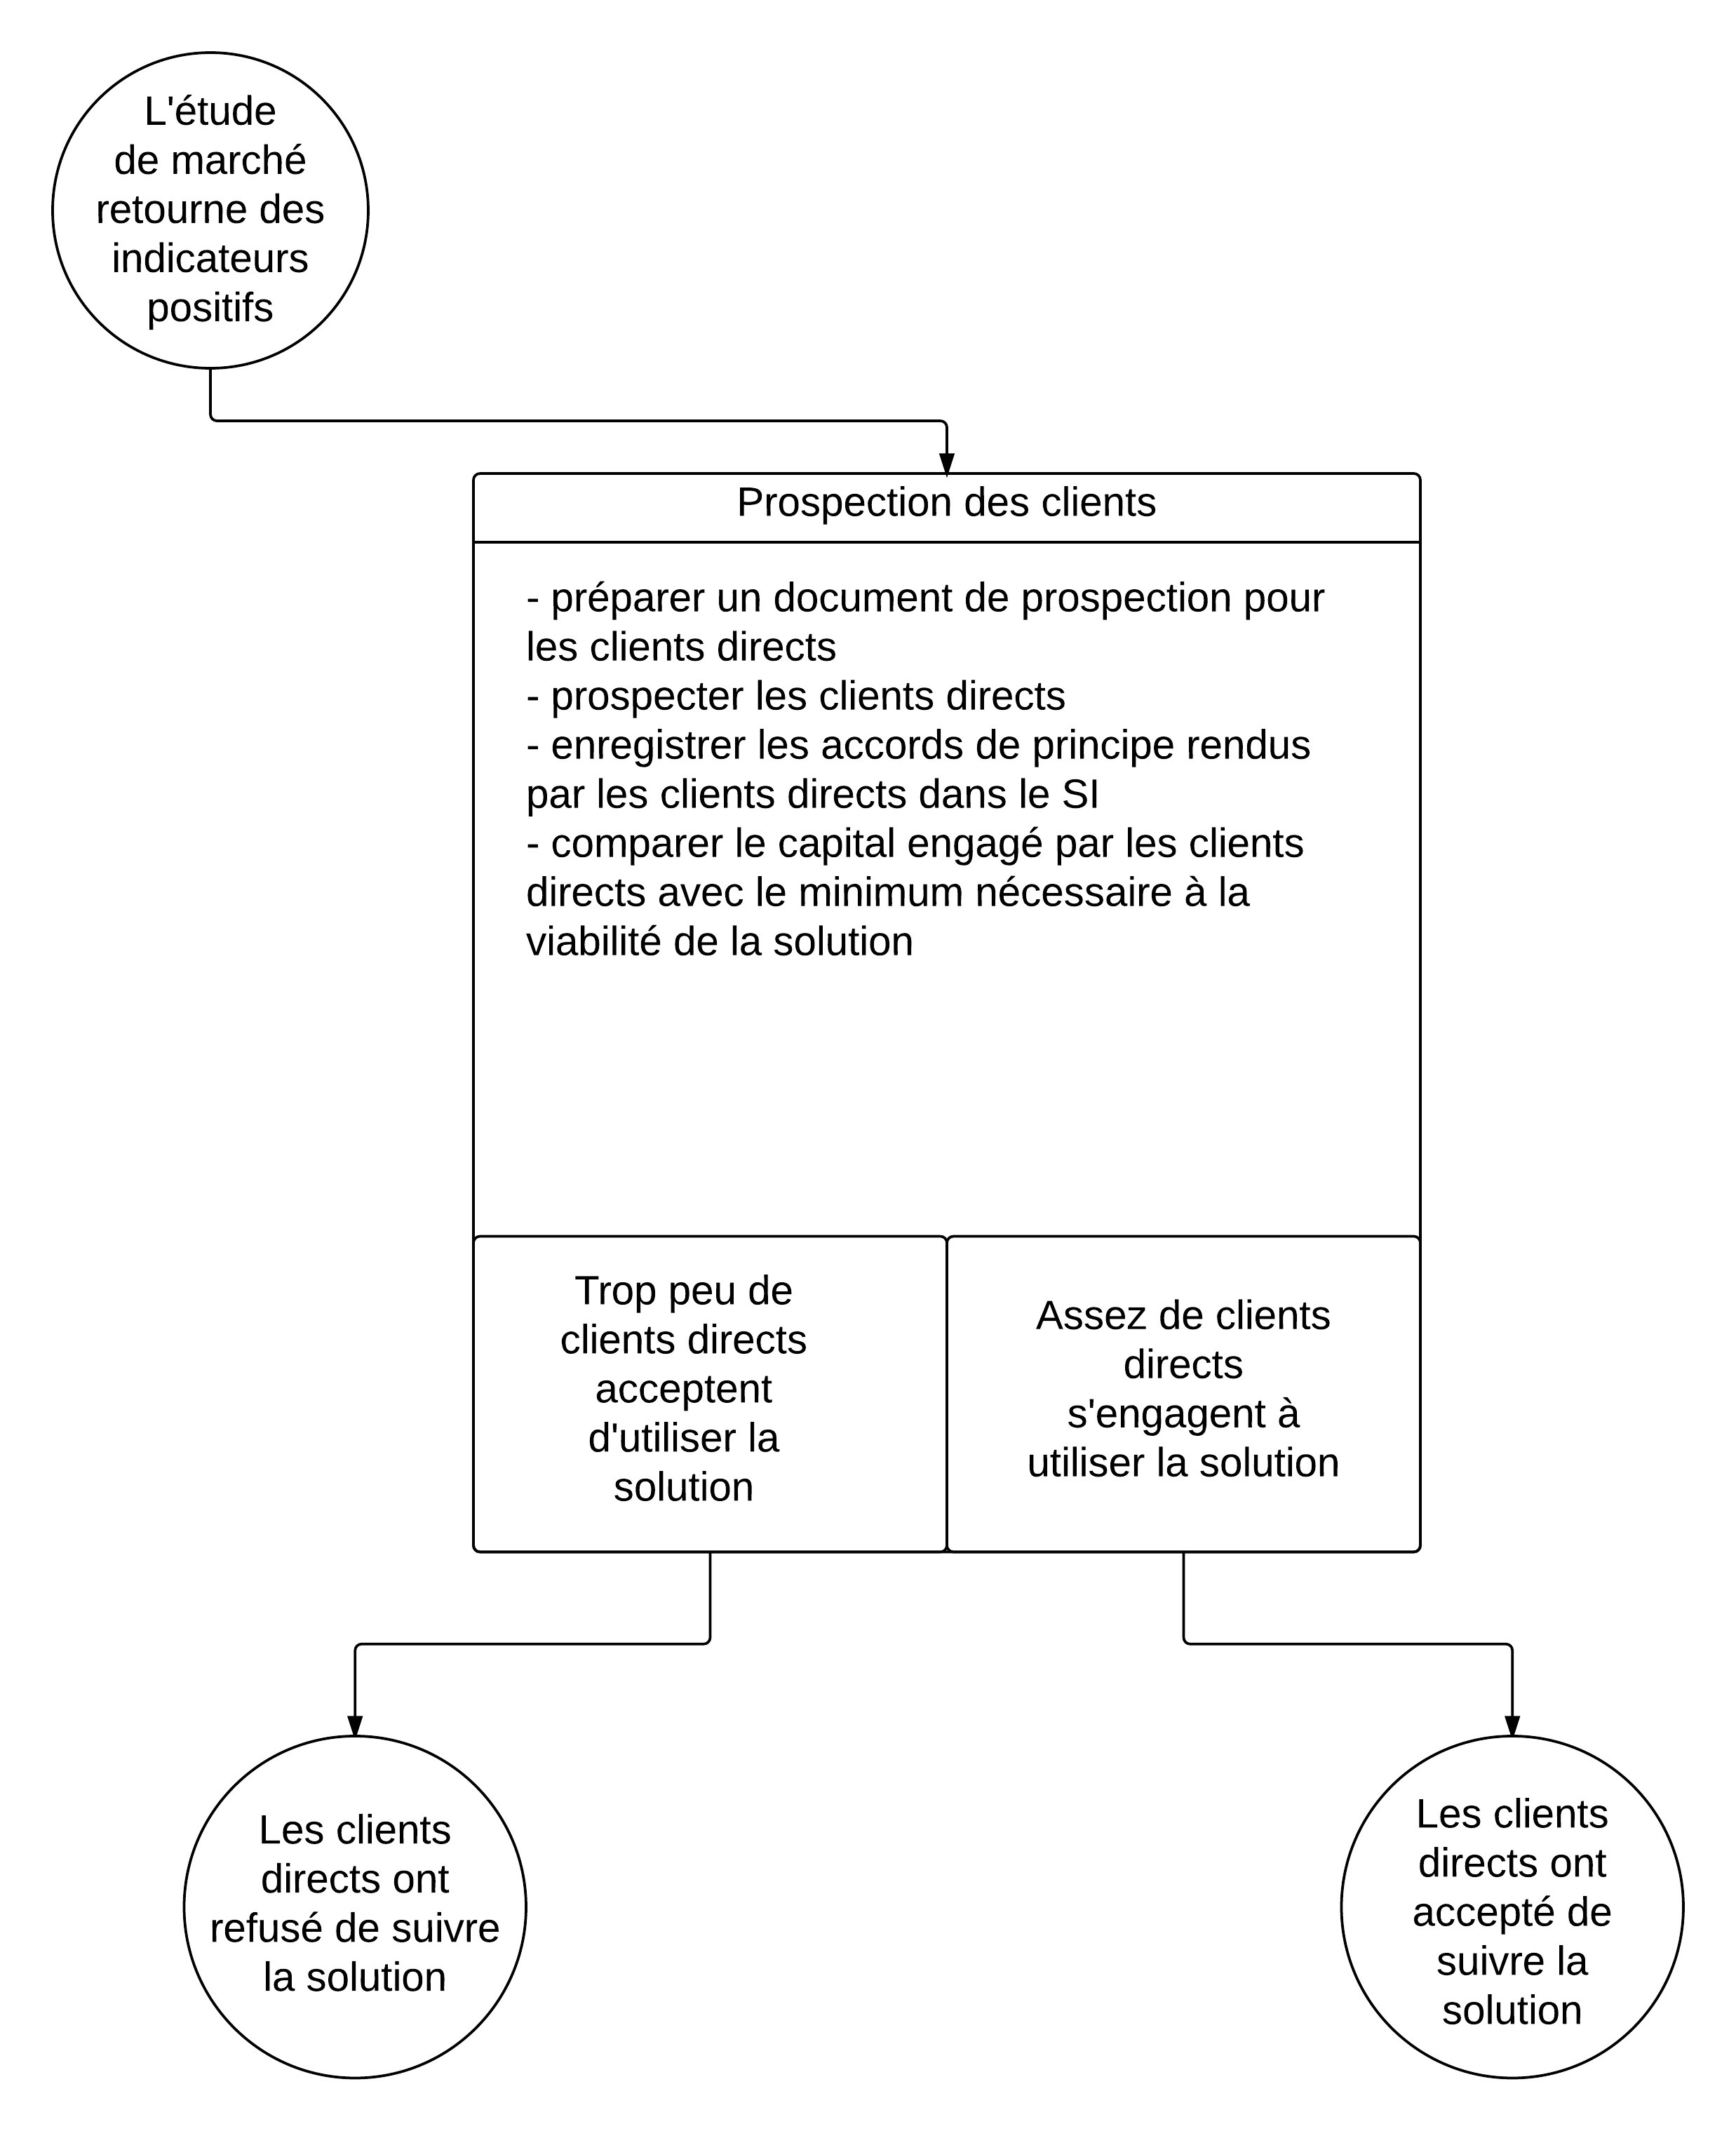
\includegraphics[width=\textwidth]{mot-prospection-clients}
    \caption{Diagramme MOT pour le traitement "Prospection des clients"}
    \label{fig:mot-prospection-clients}
\end{figure}
% \newpage

Avant toute démarche de prospection des clients directs, le service marketing
aura déjà eu à sa disposition une \textbf{étude du marché} auprès des
utilisateurs finaux afin d'avoir une confiance sur l'intérêt de la solution.
Cette dernière étude devra être effectuée en dehors de l'étude ci-présente pour
garantir sa pertinence. \\

La prospection des clients devra bien sûr être faite spécifiquement en ciblant
chaque client au mieux. Parmi les clients directs, les commerçants prospectés
devront être choisis selon l'application de la solution à leur fonctionnement.
Les commerçants concernés seront détaillés dans le document \textbf{Business
plan}.

\end{document}
